\documentclass[conference]{IEEEtran}
\IEEEoverridecommandlockouts
% The preceding line is only needed to identify funding in the first footnote. If that is unneeded, please comment it out.
\usepackage{cite}
\usepackage{amsmath,amssymb,amsfonts}
\usepackage{algorithmic}
\usepackage{graphicx}
\usepackage{textcomp}
\usepackage{xcolor}
\def\BibTeX{{\rm B\kern-.05em{\sc i\kern-.025em b}\kern-.08em
    T\kern-.1667em\lower.7ex\hbox{E}\kern-.125emX}}
\begin{document}

\title{Deep Learning for Lumbar Spine Classification}

\author{\IEEEauthorblockN{Arjun Ashok}
\IEEEauthorblockA{\textit{Department of Computer Science, Statistics} \\
\textit{University of California, Davis}\\
Davis, USA\\
arjun3.ashok@gmail.com}
\and
\IEEEauthorblockN{Zhian Li}
\IEEEauthorblockA{\textit{dept. name of organization (of Aff.)} \\
\textit{University of California, Davis}\\
Davis, USA \\
email address or ORCID}
\and
\IEEEauthorblockN{Ayush Tripathi}
\IEEEauthorblockA{\textit{Department of Computer Science} \\
\textit{University of California, Davis}\\
Davis, USA \\
atripathi7783@gmail.com}
}

\maketitle


%%%%%%%%%%%%%%%%%%%%%%%%%%%%%%%%%%%%%%%%%%%%%%%%%%
\begin{abstract}
As deep learning becomes increasingly prevalent across industries, research into how such models can assist medical professionals in diagnosing conditions has become a popular endeavor. In this project, we explored how baseline vision models (e.g. classic CNN), state-of-the-art vision models (ResNet, Vision Transformer), and novel model architectures (Kolmogorov-Arnold Networks) stack up against each other in the context of diagnosing the severity of lumbar conditions via radiology imagery provided by RSNA. We then compare our architectures' results against prior work using ResNets to generate a more thorough conclusion on what models may fair better in future applications of deep learning in diagnosis from the perspective of performance and interpretability.
\end{abstract}

\begin{IEEEkeywords}
Deep Learning, Medical Imaging, CNN, ResNet, Transformer, KAN
\end{IEEEkeywords}


%%%%%%%%%%%%%%%%%%%%%%%%%%%%%%%%%%%%%%%%%%%%%%%%%%
\section{Introduction}
\subsection{Problem}
Lower back pain is the leading cause of disability in the world, impacting over 619 million people world-wide \cite{WHO}. Spondylosis, in particular, encapsulates a set of degenerative spinal conditions that can be diagnosed via Magnetic Resonance Imaging (MRI) as follows;
\begin{itemize}
    \item Left Neural Foraminal Narrowing
    \item Right Neural Foraminal Narrowing
    \item Left Subarticular Stenosis
    \item Right Subarticular Stenosis
    \item Spinal Canal Stenosis
\end{itemize}

Although widespread in its effect, Spondylosis often goes undiagnosed and untreated, leading to chronic health issues for those suffering from lower back pain. Accordingly, there exists a strong need for diagnosing these conditions early, accurately, and in an explainable way across all 5 subsets of the condition.

\subsection{Motivation}
As the application of deep learning for aiding medical diagnoses surges, the importance of introducing accurate and interpretable models becomes increasingly relevant. In fact, prior to a competition hosted by the Radiologists Society of North America (RSNA) for using deep learning on this dataset, no research or intense application of machine learning for this subset of conditions has been developed.

As such, there is a strong need for the following:
\begin{itemize}
    \item \textbf{Accurate Diagnosis}: building upon prior research to produce a more accurate model fit for real-world deployment.
    
    \item \textbf{Explainability}: limit model complexity to retain interpretability for diagnosticians leveraging the pipeline; after all, an accurate diagnosis is worthless without sufficient explanation of why.

    \item \textbf{Comparison for Future Endeavors}: in the process of constructing the most capable pipeline for this task, we want to explore a variety of architectures and approaches to conclude which is the most promising for future work to explore, both within this problem and in related contexts.
\end{itemize}


\subsection{Prior Work}
As previously touched on, the majority of previous research into this problem comes from the recent competition hosted by RSNA on Kaggle. Prior work has thus far failed to achieve remarkably good performance. The large majority of proposed models average a weighted-log loss of $~0.36$ at best. We'll reference back to this loss as our baseline performance measurement.

Related work also includes work on the individual architectures employed \cite{convnet}, \cite{resnet}, \cite{transformer}, \cite{unet}, and \cite{kan}, although they generally touch less on downstream application and focus more on the core model design.

%%%%%%%%%%%%%%%%%%%%%%%%%%%%%%%%%%%%%%%%%%%%%%%%%%
\section{Dataset}
\subsection{Source}
As mentioned previously, we leverage the dataset collected by the Radiological Society of North America (RSNA) in partnership with the American Society of Neuroradiology (ASNR). The dataset tracks 1975 patients, each with multiple scans across multiple angles.

\begin{figure}
    \centering
    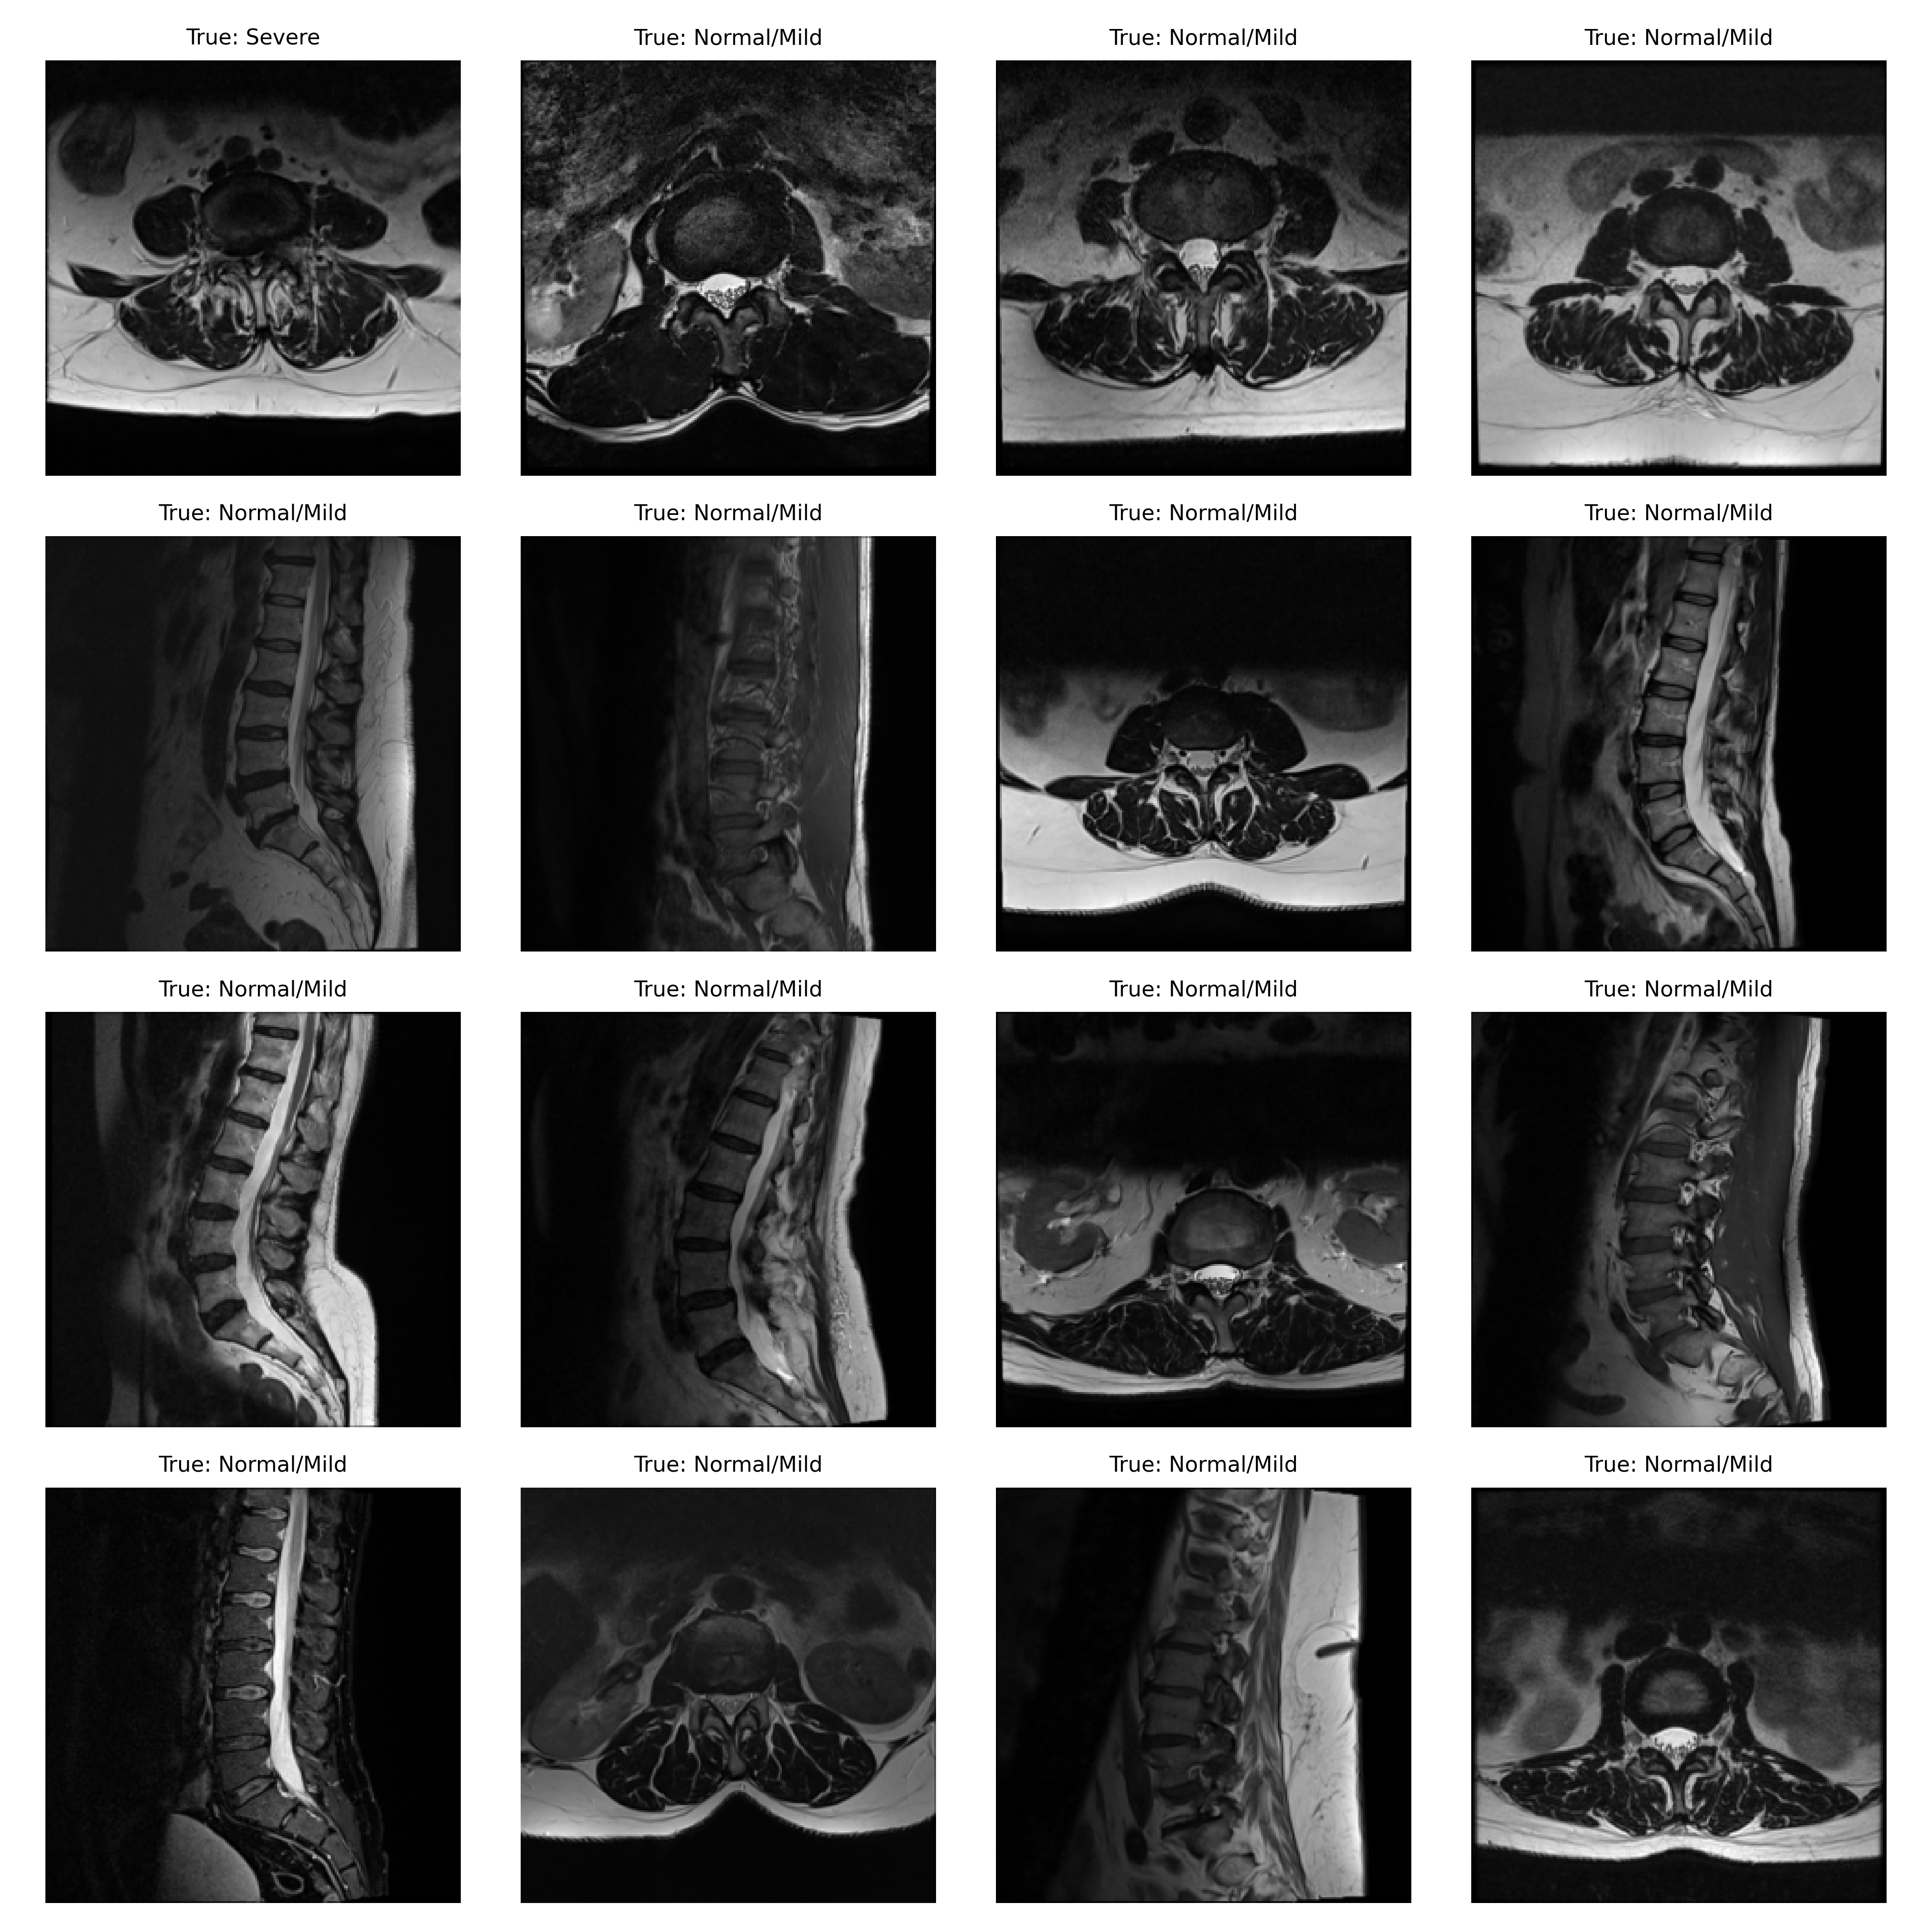
\includegraphics[width=0.8\linewidth]{visuals/dataset_sample_no_preds.png}
    \caption{A quick sampling of the dataset (un-processed except for resizing) we use and their corresponding target labels.}
    \label{fig:data_sample}
\end{figure}

Each imaging study in the dataset includes the target severity scores (Normal/Mild -- 0, Moderate -- 1, Severe -- 2) and intervertebral disc level information (L1/L2, L2/L3, L3/L4, L4/L5, L5/S1). We only leverage the severity scores for the classification task, thus requiring only one classification head of 3 nodes.

\subsection{Transforms}
Prior to training, we briefly pre-process the MRI data across all models to improve performance remain consistent in our comparison. The transforms we conduct are as follows:
\begin{enumerate}
    \item \textbf{Resize}: we resize all images to $224 \times 224$ to ensure a consistent input for all models--this allows an even comparison for the downstream computational efficiency and further standardizes the input.

    \item \textbf{Normalize}: we normalize all images such that every channel (just one in this case since MRI images are grayscale) is distributed with mean pixel brightness of 0.5 and standard deviation of 0.5. Not only does this aid with consistency across each batch, but we get the additional benefit of a model less sensitive to learning rate since all inputs will adhere to a set range of values. The observed downstream impact is a faster, stabler convergence across all architectures during empirical testing.
\end{enumerate}

Respectively, we leverage $\approx 70\%$, $\approx 10\%$, $\approx 20\%$ of the data for training, validation, and testing.


%%%%%%%%%%%%%%%%%%%%%%%%%%%%%%%%%%%%%%%%%%%%%%%%%%
\section{Model Architectures}
\subsection{Convolutional Neural Network (CNN)} \label{sec:CNN}
Convolutional Neural Networks have become the de-facto architecture employed with image processing tasks in recent years. Their flexibility in learning filters specific for a given task rather than need pre-built/manually specified convolutional kernels allows them to outperform traditional MLPs quite effectively.

Our deployed architecture makes use of two fundamental blocks:
\begin{enumerate}
    \item \textbf{Convolutional Process}: each convolutional process
    consists of a 2D-convolutional layer ($7 \times 7$ kernel), a ReLU activation, and a 2D-Max-Pooling ($2 \times 2$ kernel). We stack 3 convolutional processes to conduct sufficient feature extraction (with 8, 16, then 32 channel outputs respectively).
    
    \item \textbf{Multi-Layer Perceptron (MLP)}: we feed the last convolutional process' outputs into a traditional multi-layer perceptron head of 3 fully-connected, linear layers to perform the classification. Recall our output layer will have 3 nodes, one for each severity.
\end{enumerate}

\subsection{Modified Convolutional Neural Network (MCNN)}
The most recent trend in deep learning for computer vision is attention-based networks, i.e. vision transformers. To continue maintaing its relevancy, one group of researchers have augmented ConvNet to produce ConvNeXt: a CNN-based architecture that lends some architectural decisions from attention-based models \cite{convnet}. Due to the substantially different training approach they utilized, we opted to use a subset of their augmentations on ConvNet to apply on our own CNN \ref{sec:CNN}:
\begin{itemize}
    \item \textbf{Activation Functions}: rather than applying ReLU after each operation, we utilize a single GeLU operation in every convolutional process \cite{convnet}.
    
    \item \textbf{Normalization}: taking inspiration from vision transformers, we utilize layer normalization over batch normalization \cite{convnet}.
\end{itemize}

Though these changes appear small, their downstream impact has proven rewarding in prior work and may encourage similar borrowing in future work \cite{convnet}.

\subsection{Residual Neural Network (ResNet)}
ResNet was first developed by Microsoft Research (MSR) with the goal of deepening neural architectures \cite{resnet}. Previously, models with deep hidden layers would suffer from the vanishing gradient problem, i.e. gradients would start to approach zero as backpropagation moved away from the output layers. To remedy this, ResNet relies on learning a function $F(x)$ for the input $x$ such that $H(x) = F(x) + x$. More succinctly, the model learns to augment the input over each residual block rather than transforming the whole input as in other architectures. Thus, each residual block will have the output of the previous residual block added to its own output \cite{resnet}.

With this mechanism, ResNet architectures can be much deeper while retaining trainability. In our implementation of ResNet, we leverage the ResNet-18 architecture (18 layer CNN) without pre-training.

\subsection{Vision Transformer (VIT)}
Transformers were initially developed by Google Brain for processing and generating large sequences of data, particularly in text-related tasks such as translation \cite{transformer}. Recent work, however, has explored the use of transformers in vision settings--unsurprising since convolution has similarly proved useful for text-related tasks \cite{VIT} \cite{transformer}. The vision transformer has proved to be extremely effective at learning context within images, matching the performance of state-of-the-art models at a fraction of the compute \cite{VIT}.

Briefly, vision transformers work by dividing an image into a grid of smaller cells, where each cell can be thought of as a token. As with text-related tasks, attention blocks are highly effective at making associations between tokens, allowing the vision transformer to leverage broader context across all grid cells. A convolutional network, in comparison, inherently relies on the surrounding region of a pixel to extract information, thereby prone to ignoring important context that is not spatially close-by.

For our implementation of the vision transformer, we built a backbone of 


\subsection{Convolutional Kolmogorov-Arnold Network (CKAN)}
Kolmogorov-Arnold Networks are an alternative basis to the perceptron-learning networks that have thus far powered deep learning architectures.

Briefly, deep learning is based on approximations--the objective of neural networks is to learn a manifold of some kind, i.e. approximate a function \cite{mlp_approx_thm}. The Universal Approximation Theorem enabled the Multi-Layer Perceptron architecture by roughly proving that feed-forward networks with non-polynomial activations can map between two Euclidean spaces (i.e. approximate any function) \cite{mlp_approx_thm}. Note here that this doesn't explicitly prove a method of convergence (global minimum), although backpropagation tends to estimate parameters well enough for practical use (local minimum) \cite{mlp_approx_thm}.

However, an alternative basis has recently been explored with the Kolmogorov-Arnold Representation Theorem \cite{kan}. The theorem roughly states that any multivariate, continuous function can be decomposed into a \textit{finite} sum of single-variable, continuous functions \cite{kan_approx_thm}. The most promising application of this basis has been in learning activation functions as splines rather than a set function \cite{kan}. In addition to enabling a smaller network to emulate the performance of a larger MLP, this approach allows for increased interpretability by way of these learned splines \cite{kan}. This is analagous to a learned kernel in CNNs for better performance and interpretation.

Due to its relatively new deployment, we opted to simply replace some of MLP layers from our MCNN model to these spline linear layers. Thus, our best point of comparison for KAN spline layers versus traditional MLP layers will be the MCNN.


\subsection{Model Interpretation}
For convolutional architectures (e.g. CNN, MCNN, CKAN, ResNet), we can leverage a popular interpretation technique Grad-Cam to interpret the model. Grad-Cam works by taking the gradients (i.e. back-propagating) from the target class' node in the output layer to the final convolutional layer to highlight important parts of the image for triggering the output activation \cite{gradcam}.


\subsection{Future Explorations}
To ensure the cleanest comparison across architectures (and deal with time and computation constraints), we opted against integrating some potentially beneficial model-agnostic techniques. We highlight them here as future paths of exploration:
\begin{itemize}
    \item \textbf{Data Augmentation}: given the controlled environment of an MRI machine, most augmentations would likely not apply to our context without causing more harm than good for model training. However, some techniques such as jitter, horizontal flips, and slight blurring may help the model in deployment since patients may get restless during the long imaging process of an MRI and/or be place in either orientation.

    \item \textbf{Pre-Training}: across all model, pre-training via a related task (e.g. X-ray imaging diagnosis) or even a generic task (e.g. ImageNet) may benefit the model's downstream performance. Exploring certain pre-text (pseudo) tasks may also be a worthwhile path to explore.

    \item \textbf{Region Proposal}: although RPNs have proven highly effective in reducing overhead computation and improving bounding box regression, their inclusion in our models seem to distract from the simpler classification task. That being said, if future work aimed to provide doctor's with a region of interest to inspect (i.e. a bounding box output), an RPN would certainly warrant further consideration.

    \item \textbf{U-Net (UNET)}: the U-Net is a convolutional architecture primarily developed for biological segmentation with limited annotated data points \cite{unet}. Although the underlying backbone could potentially be leveraged for classification, computational constraints became apparent during experimentation. For future work, we recommend utilizing this model for segmenting the images for further interpretability for the diagnosticians.
\end{itemize}


%%%%%%%%%%%%%%%%%%%%%%%%%%%%%%%%%%%%%%%%%%%%%%%%%%
\section{Results}
\subsection{Computational Efficiency}
- how fast was each model to train
- how fast is each model in prediction
- table comparing models
- convergence graphs go here

\subsection{Performance}
- table comparing how accurate each model is
- show example of misclassified images, correctly classified images

\subsection{Model Interpretation}
- what can each architecture teach us about the diagnosing process?


%%%%%%%%%%%%%%%%%%%%%%%%%%%%%%%%%%%%%%%%%%%%%%%%%%
\section{Conclusion}
- how did we end up comparing to the models we wanted to outperform?
- any lessons learned?
- future goals / building on this research
- threats to validity


%%%%%%%%%%%%%%%%%%%%%%%%%%%%%%%%%%%%%%%%%%%%%%%%%%
\section{Authors \& Acknowledgment}
\begin{itemize}
    \item \textbf{Arjun Ashok}: project lead. Built core model architecture \& methods, implemented CNN/MCNN/KAN/ResNet, researched architectures, built model interpretation via GradCam. Wrote abstract, introduction, dataset, model architecture, and parts of results \& conclusion
    \item \textbf{Zhian Li}: contributions go here
    \item \textbf{Ayush Tripathi}: contributions go here
\end{itemize}

We'd also like to extend our appreciation to Professor Hamed Pirsiavash for an informative course and the TA's of ECS 174, Raymond Kang and Kossar Pourahmadi-Meibodi for their efforts in teaching.


%%%%%%%%%%%%%%%%%%%%%%%%%%%%%%%%%%%%%%%%%%%%%%%%%%
\appendix
\subsection{Computation}
All compute was done on one of two machines:
\begin{enumerate}
    \item Nvidia 4080 Super, AMD 9900X
    \item Nvidia 4070 Super, AMD 9800X3D
\end{enumerate}

We leveraged a CUDA-enabled PyTorch compilation for all models except CKAN--the CKAN library we've used is unable to run on GPUs yet, so we trained purely on CPU.

\subsection{Hyperparameters}
All models used the same set of initial hyperparameters:
\begin{itemize}
    \item \textbf{Epochs for Early Stopping}: 5. All models employed early stopping for training to limit overfitting. This parameter controls how many epochs we would wait with no improvement in validation performance before making the decision to early stop.
    
    \item \textbf{Number of Epochs}: 30. We trained all models up to 30 epochs, although in most cases we needed less to converge before early stopping kicked in.

    \item \textbf{Batch Size}: 32
    
    \item \textbf{Learning Rate}: $1 \times 10^{-4}$
    
    \item \textbf{Momentum}: 0.7. We don't pass this parameter in since we leverage the Adam optimizer
    
    \item \textbf{Batch Size}: 32

    \item \textbf{Dropout Rate}: 0.3. Some models don't implement dropout.

    \item \textbf{Optimizer}: Adam

    \item \textbf{Loss Criterion}: Cross Entropy Loss

    \item \textbf{Classification Function}: Softmax. The alternative is to use sigmoid.
\end{itemize}

The vision transformer (VIT) has additional default parameters not mentioned here.

%%%%%%%%%%%%%%%%%%%%%%%%%%%%%%%%%%%%%%%%%%%%%%%%%%
\bibliographystyle{plain}
\bibliography{refs}

\end{document}
